\parindent=1cm %красная строка
\begin{center}
	
	\section{Понятие <<цифровой угрозы>> , новые цифровые угрозы}
	
\end{center}

Дадим определение понятию << цифровая угроза >> и рассмотрим их основные виды.
\subsection{Определение}


	\textbf{Цифровая угроза} -- совокупность условий и факторов, создающих опасность нарушения информационной безопасности  в контексте нарушения тайны связи.%LITER: https://ru.wikipedia.org/wiki/%D0%A3%D0%B3%D1%80%D0%BE%D0%B7%D1%8B_%D0%B8%D0%BD%D1%84%D0%BE%D1%80%D0%BC%D0%B0%D1%86%D0%B8%D0%BE%D0%BD%D0%BD%D0%BE%D0%B9_%D0%B1%D0%B5%D0%B7%D0%BE%D0%BF%D0%B0%D1%81%D0%BD%D0%BE%D1%81%D1%82%D0%B8#%D0%9B%D0%B8%D1%82%D0%B5%D1%80%D0%B0%D1%82%D1%83%D1%80%D0%B0
<<Цифровая угроза>> является частным случаем \textit{угрозы информационной безопасности} -- угрозой конфиденциальности (неправомерный доступ к информации) и угрозой доступности (осуществление действий, делающих невозможным или затрудняющих доступ к ресурсам информационной системы). 

Угрозы называются <<\textbf{новыми}>>, так как их бурное развитие и рост числа инцидентов произошли в последние 10-15 лет и сами угрозы постоянно меняются, увеличивается их количество.  

\subsection{Основные виды угроз в частном секторе}

%Основными причинами  утечки и перехвата сообщений являются SpyWare (вирусы), целенаправленные атаки на протоколы и средства связи, халатность отправителя, состоящая в использовании недоверенных  сетей и средств. Рассмотрим каждую причину подробнее.
	Основными видами новых цифровых  угроз являются  утечки и перехваты сообщений, происходящие с помощью  SpyWare (подмножество вирусов),  целенаправленных атак  на протоколы и средства связи,атак на криптографические протоколы, халатность отправителя, состоящая в использовании недоверенных  сетей и средств. Рассмотрим каждый вид  подробнее.
	
	\textbf{SpyWare}. Вирус в классическом понимании представляет собой программы, целенаправленно создающие свои копии и передающие их по разным каналам связи на другие устройства , способные внедряться в код других программ, загрузочные секторы жёстких дисков. При этом основной функцией вируса является саморепликация и распространение, а модификация  работы аппаратно-программных комплексов -- всего лишь сопутствующая функция. SpyWare (сокр от Spy Software -- <<Шпионское программное обеспечение>>) представляет отдельный класс вредоносного ПО, лишенный репликативных свойств вируса. Основным назначением SpyWare является мониторинг, сохранение и передача злоумышленнику данных о работе ПО, пользовательской активности и самом пользователе  на заражённом устройстве. Установка таких программ происходит скрытно и не предполагает возможности пользователя следить за работой такой программы или её удаления.     Для перехвата сообщений используются кейлоггеры(keyloggers), осуществляющие логирование всех нажатых клавиш, скрин-скраперы(screen scrapers), создающие снимки экрана через заданный интервал времени или по наступлению события, и обобщенные следящие программы, способные перехватывать содержимое почтовых программ и веб-страниц, открытых на заражённом устройстве, с помощью post-get запросов и автоматизированных средств взаимодействия с веб-браузером таких как Selenium. 
	
	
	К SpyWare не относятся программы, добровольно установленные пользователем и применяющиеся на совершенно  законных основаниях  для мониторинга состояния устройства, оказания удалённой технической поддержки,исследования защищённости компьютерных систем, желаемых пользователем персонализации и обновления компонентов ПО \cite{MailWare1}. %LITER https://ru.wikipedia.org/wiki/Spyware
	%LITER https://sonikelf.ru/chto-takoe-spyware-i-kak-s-etim-borotsya/
	
	Рассмотрим отдельно самого распространённого представителя SpyWare -- \textbf{кейлоггер} -- программный или аппаратный комплекс, регистрирующий взаимодействие пользователя с устройствами ввода-вывода, в классическом случае -- с клавиатурой и мышкой\cite{MailWare2}. %LITER https://sonikelf.ru/keylogger-chto-eto-ili-shpionazh-chistoj-vody-na-pk/ 
	Первые кейлоггеры появились в эпоху MS-DOS и представляли собой перехватчик прерывания int  16h \cite{INT16H}.	 %LITER http://www.codenet.ru/progr/dos/int_0015.php
	
	
	Современные компьютеры, работающие в protected mode, не дают программисту доступ к таким низкоуровневым возможностям, поэтому теперь в основе современных кейлоггеров лежит использование \textbf{хуков} -- технологии, позволяющей изменить стандартное поведение тех или иных компонентов информационной системы. Обычно для этого используются компоненты Win32API: WH\_Keyboard, WH\_JOURNALRECORD. Преимущество последнего заключается в отсутствии необходимости использования DLL, что упрощает распространение вируса через компьютерные сети. Недостатком использования хуков является легкая обнаружимость DLL с хуком, так как для перехвата нажатий DLL отображается в адресное пространство всех GUI-процессов. 
	
	
	Второй популярной методикой является циклический опрос состояния клавиатуры с высокой скоростью. Преимуществом является меньшая заметность кейлоггера, однако присутствует значительный недостаток -- необходимость очень частого опроса клавиатуры, примерно 10-20 опросов в секунду -- современные ОС могут не выделить процессу с низким приоритетов столько ресурсов или не предоставлять доступ с такой частотой. 
	
	Третий способ является одним из наиболее эффективных и представляет собой кейлоггер уровня драйвера. В таком случае кейлоггер является частью драйвера, незаметен для большинства антивирусов, не может быть удален без потери функциональности клавиатуры. Также возможна реализация драйвера-фильтра, являющегося прослойкой между настоящим драйвером и ОС. Также к низкоуровневым кейлоггерам может быть отнесен руткит, перехватывающий обмен  csrss.exe (Server Client Runtime Subsystem)\cite{Csrss}.
	%LITER http://fb.ru/article/195605/csrss-exe---chto-eto-csrss-exe-gruzit-protsessor-kak-lechit
	%GRAPH:  https://sonikelf.ru/attach/img/1351669030-clip-9kb.jpg  
		
	
	\begin{figure*}[h!]
		\centering{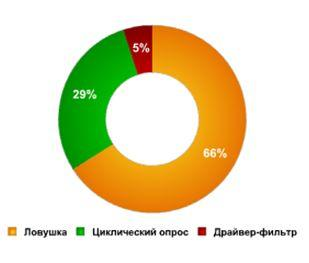
\includegraphics[scale=3]{KeyLog.jpg}}
		\caption{ Диаграмма распределения популярности реализаций кейлоггеров по данным портала sonikelf.ru.}
	\end{figure*} 
	В последнее время на рынке гаджетов появились аппаратные клавиатурные устройства, имеющие сходный с программным кейлоггером   функционал, представляющие собой USB-флешки, регистрирующие нажатия клавиш и записывающие их на собственную память. Такое устройство может автономно работать достаточно долго. Если предположить, что средний менеджер нажимает примерно 23000 клавиши в день(обозначим константой ApD), один символ занимает 1 килобайт памяти, что является намеренным упрощением, (обозначен переменной  S) \cite{PressPerDay}  %LITER https://habr.com/company/io/blog/263795/ 
	и взять емкость запоминающего устройства 16Gb (обозначим константой Mem), то памяти хватит на $ \frac{Mem}{Apd * S } = \frac{16 Gb}{23000*9,54*10^{-7} Gb} $ = 727 дней автономной работы. 
	
	\textbf{Атаки на протоколы и средства связи}
	
	
	Большинство атак на протоколы связи основаны на принципе \textbf{<<Человек в середине>>} или <<Атака посредника>>  (<<Man in the midle>>, MITM). В основе такой атаки лежит перехват сообщений на линии коммуникации между отправителем  и абонементом.  При этом возможны два метода атаки: пассивное прослушивание заключается в перехвате и анализе сообщений, если они зашифрованы, активная атака предполагает перехват, анализ сообщений, взлом криптографических алгоритмов, если такие используются, изменение содержимого сообщения и/или предотвращение передачи без разрушения канала связи. 
	
	Современные протоколы коммуникации используют различные криптографические протоколы, при этом шифрование происходит непосредственно на устройствах, то есть через коммуникационные сети передается уже зашифрованное сообщение, которое невозможно просто прочитать или модифицировать, не взломав ключ шифрования или не использовав другую уязвимость, поэтому будут рассмотрены именно активные методы атаки. 
	
	Пример атаки на алгоритмическом языке: Алиса хочет передать сообщение Бобу, Мэлори хочет перехватить и, возможно, изменить его так, чтобы Боб получил  злонамеренно ошибочное сообщение:
	\begin{enumerate}
		\item Алиса отправляет сообщение Бобу,  сообщение перехватывает Мэлори;
		\item Мэлори пересылает сообщение Бобу, который не знает, что сообщение не от Алисы;
		\item Боб посылает свой ключ;
		\item Мэлори подменяет ключ Боба своим, затем  пересылает сообщение Алисе;
		\item Алиса принимает сообщение, шифрует свое сообщение ключом Мэлори, который считает ключом Боба и  что только он сможет расшифровать его, отправляет сообщение Бобу;
		\item Мэлори перехватывает сообщение, шифрованное ключом Мэлори (лже-Боба), модифицирует его, шифрует ключом Боба и отправляет Бобу;
		\item Теперь Мэлори может модифицировать сообщения  обеих сторон, даже если те решат изменить ключи.
	\end{enumerate}
	Атаки типа MIT показывают важность точного подтверждения того, что обе стороны используют настоящие открытые ключи: у стороны A открытый ключ стороны B и у стороны B открытый ключ A. Если такое подтверждение не используется, то канал может быть атакован по принципу MIT. 
	
	\textbf{Атаки на криптографические протоколы}
	Криптографические протоколы в зависимости от сложности  решают одну или несколько   задач: шифрование/дешифрование, создание электронной цифровой подписи (ЭЦП, digital signature, DS), идентификация/аутентификация, аутентифицированного распределение ключей. Атаки на протоколы можно разделить на пассивные и активные: при пассивных атаках взломщик(криптоаналитик) не участвует в протоколах, только следит за протоколом и пытается раздобыть ценную информацию на основе перехватываемого шифротекста; при активных атаках   аналитик пытается изменить протокол к собственной выгоде и для этой цели активный взломщик может выдавать себя за другого человека, повторять или 	 заменять сообщения, разрывать линию, модифицировать информацию. В  целом, классификация атак на криптографические протоколы совпадает с классификацией атак на сетевые коммуникационные протоколы.
	
	Рассмотрим самые широко известные  атаки на криптографические протоколы \cite{CryproAttackDiscribe} : %LITER: http://myunivercity.ru/%D0%9F%D1%80%D0%BE%D0%B3%D1%80%D0%B0%D0%BC%D0%BC%D0%B8%D1%80%D0%BE%D0%B2%D0%B0%D0%BD%D0%B8%D0%B5_%D0%B8_%D0%BA%D0%BE%D0%BC%D0%BF%D1%8C%D1%8E%D1%82%D0%B5%D1%80%D1%8B/%D0%90%D1%82%D0%B0%D0%BA%D0%B8_%D0%BD%D0%B0_%D0%BA%D1%80%D0%B8%D0%BF%D1%82%D0%BE%D0%B3%D1%80%D0%B0%D1%84%D0%B8%D1%87%D0%B5%D1%81%D0%BA%D0%B8%D0%B5_%D0%BF%D1%80%D0%BE%D1%82%D0%BE%D0%BA%D0%BE%D0%BB%D1%8B/361_43116_%D1%81%D1%82%D1%80%D0%B0%D0%BD%D0%B8%D1%86%D0%B01.html
	
	
	\textbf{Подмена}. Метод атаки заключается в подмене одного контрагента переписки другим. Аналитик,  выступая от имени одной стороны коммуникации, полностью имитирует её действия, получает сообщения определенного формата, необходимые для анализа шифротекста и подделки определенных шагов протокола.
	
	\textbf{Повторное навязывание сообщения} (replay attack). Атака основана на повторной передаче ранее переданных в текущей или прошедших сессиях  сообщений или частей сообщения. Например, повторная передача  информации проведенного ранее протокола идентификации/аутентификации может привести к повторной успешной идентификации/аутентификации атакующего как настоящего контрагента общения. Такая атака также может быть использована в протоколах передачи ключей для навязывания ранее использованного сеансового ключа и известна как атака на основе новизны (freshness attack).
	
	\textbf{Параллельная атака} (parallel-session attack). Аналитик открывает несколько параллельных сессий, при этом сообщения и полученные аналитиком  данные  из одного сеанса используются для   анализа шифротекста и ключей другого сеанса.
	
	\textbf{Атака с использованием специально подобранных текстов}. Атака на post-get запросы, при которой аналитик по определенному правилу подбирает запросы и их содержимое с целью анализа долговременного ключа собеседника.
	
	\textbf{Атака по известному сеансовому ключу} (known-key attack). Заключается в получении долговременных ключей, новых сессионных ключей или установлении алгоритма, используемого для генерации новых ключей по известному использованному ранее сессионному ключу.
	
	\textbf{Использование уязвимостей  алгоритма или ошибок реализации }. 	В атаках такого типа аналитик ищет уязвимости, связанные с алгоритмом или ошибки реализации. Такая атака может давать самые долговременные и серьезные результаты, так как для успешного отражения контрагентам необходимо узнать о компрометации используемого алгоритма и внести исправления в алгоритм и его реализацию. Однако, такая атака является достаточно затруднительной для аналитика, так как требует реверс-инжиниринга  алгоритма и его реализации, что может быть затруднительно в реальных коммуникационных сетях, где аналитику доступен только шифротекст и время отправки сообщения.\\
	
	Перечисленные выше угрозы относятся к частному и корпоративному общению, при этом государство или несколько государств не являются  стороной коммуникации или криптоаналитиком. Ниже рассмотрим теоретические ситуации и конкретные прецеденты, когда государство (под <<государством>> далее понимается совокупность судебной, законодательной и исполнительной властей конкретного государства) является криптоаналитиком или пособником аналитика по отношению к своим или иностранным гражданам. 
	\subsection{Наблюдение и контроль  за коммуникациями  со стороны государства}
	
	Современные законотворческие инициативы  ведущих стран Европы, Америки и Азии содержат в себе идею борьбы с терроризмом, опасность которого действительно невозможно не заметить, посредством массовой перлюстрации (просмотр личной пересылаемой корреспонденции, совершаемый втайне от контрагентов) или явного анализа цифровой переписки. 
	
	Основной проблемой в контексте тайны связи является возможность недобросовестного использования полученных данных с целью шантажа или  продажи, утечки из государственных информационных систем и хранилищ. Вторым большим опасением можно считать тот факт, что для доступа к переписке разработчики ПО оставляют backdoor'ы -- дефект алгоритма,  намеренно встраиваемый  в него разработчиком и позволяющий  получить несанкционированный доступ к данным, и если такой backdoor существует, то нет никаких гарантий, что доступ к нему не будет получен третьими лицами, что попадает под <<нарушение тайны связи>> из части 1 данной работы.

	Рассмотрим такие ситуации на примерах крупнейших мировых государств:
		
	 \textbf{Китай}. КНР проводит политику массовой слежки за гражданами по всей территории страны. В рамках этой политики реализованы два масштабных проекта: 
	
	\textbf{<<Золотой щит>>} (Великий китайский фаервол). Представляет собой  систему фильтрации содержимого интернета. Разрабатывался с 1998, введен в эксплуатацию повсеместно с 2003. Включает подсистемы управления безопасностью, информирования о правонарушениях, контроля входа и выхода, мониторинга и управления трафиком.  Функции проекта: ограничения доступа к ряду иностранных сайтов, ограничение публикаций для китайских СМИ, перехват и хранение сообщений в мессенджерах.
	
	\textbf{Интернет-цензура}. Включает в себя вышеописанный <<Золотой щит>> и комплекс мер, используемых правительством КНР для перехвата сообщений в мессенджерах и других средствах коммуникации, использующих защиту данных. 	Помимо использования стандартных приемов слежки, власти КНР используют социальные приемы. Так была создана социальная сеть <<Sina Weibo>> -- собственный проект китайской компанией Sina Corp в 2009 году. Существует мнение, что Sina Corp предоставляет доступ к данным и переписке пользователей правительству КНР, при этом сами пользователи считают, что их данные находятся под надёжной защитой владельцев платформы. 
	
	Параллельно с двумя вышеупомянутыми проектами в КНР в тестовом режиме работает система \textbf{<<Система социального кредита>>} -- система постоянного анализа поведения граждан в Интернете и в повседневной жизни. При этом в качестве поощрения и наказания выступают разрешение на работу в госучреждениях, возможность получать соцобеспечение, повышенное внимание таможни, возможность покупки билетов на самолеты и поезда, право на обучение детей в частных дорогих школах  \cite{SocialCredit} \cite{SocialCredit2}. %LITER: https://chinacopyrightandmedia.wordpress.com/2014/06/14/planning-outline-for-the-construction-of-a-social-credit-system-2014-2020/ 
	%LITER: https://www.rbc.ru/business/11/12/2016/584953bb9a79477c8a7c08a7
	\\
	\begin{figure*}[h!]
		\centering{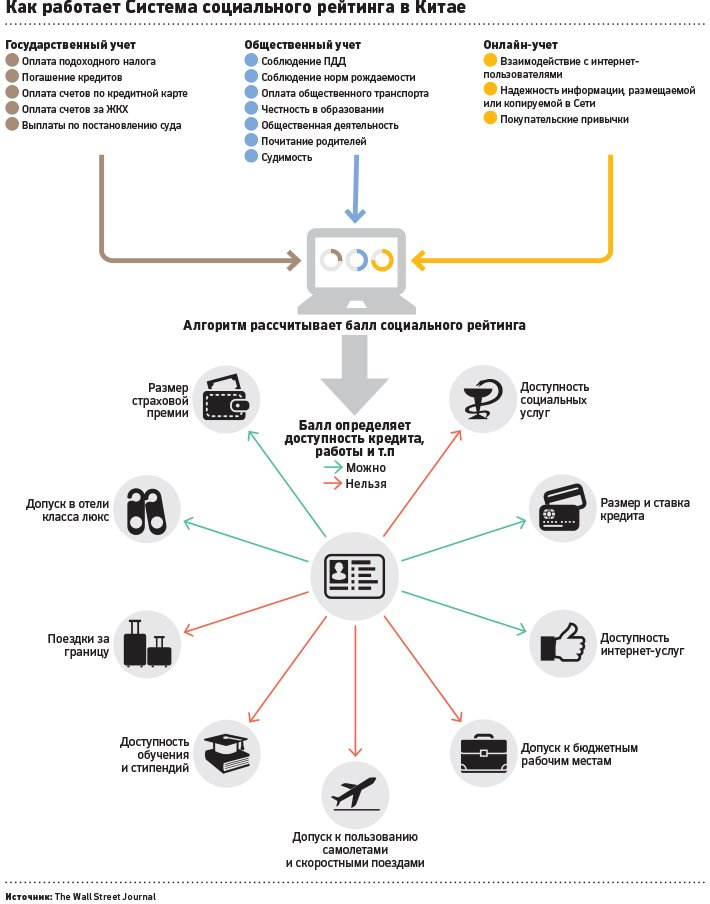
\includegraphics[scale=0.5]{ChinaControl.jpg}}
		\caption{ Принцип работы Системы Социального Рейтинга в КНР по данным РБК}
	\end{figure*} 
	\textbf{США и ЕС}. Несмотря на значительный уровень свободы слова и уважения к частной жизни, декларируемые Конституцией США, в государстве имеется широкая и мощная сеть компьютерного слежения и радиоэлектронной разведки. Задачи разведки  и слежения возложены на АНБ, ФБР, ЦРУ, Министерство финансов, Министерство обороны, Министерство юстиции и Министерство внутренней безопасности США.  
	
	Рассмотрим подробнее основные программы слежения США и ЕС:
	
	\textbf{MAINWAY}. База данных, содержащая метаданные о нескольких миллиардах телефонных звонков, совершенных через самые крупные коммуникационные компании США: AT\&T, SBC, BellSouth, Verizon. Проект находится в ведении  АНБ и имеет несколько дочерних: Stellar Wing -- программа слежения за электронной активностью, в том числе электронной почтой, телефонными звонками, активностью в Интернете, имевшая место во времена президентства Дж. Буша-младшего(2001-2009 г-г) \cite{MAINWAY1} \cite{MAINWAY2};%LITER: https://www.washingtonpost.com/investigations/us-surveillance-architecture-includes-collection-of-revealing-internet-phone-metadata/2013/06/15/e9bf004a-d511-11e2-b05f-3ea3f0e7bb5a_story.html?utm_term=.1ef7b5fd28c8 										
	%LITER:	http://thestarshollowgazette.com/2012/08/25/blowing-in-the-stellar-wind/ 	  	%LITER: https://www.webcitation.org/6I1ZBmfih
	Комната 614А -- помещение в здании провайдера AT\&T, используемое АНБ в 2003-2006 годах для перехвата интернет-коммуникаций, \cite{614-1} \cite{614-2} %LITER: https://www.wired.com/2006/05/att-whistle-blowers-evidence/								%LITER:https://www.wired.com/threatlevel/2012/03/ff_nsadatacenter/all/1
	основной принцип работы перехватывающего оборудования -- разделение  оптического сигнала, при котором 90\% мощности  используются в дальнейшем в коммуникационном оборудовании и 10\% перенаправляются на порты мониторинга для изучения и записи.
	
	\textbf{Tailored Access Operations}. Подразделение АНБ, созданное в 1997 для пассивного и активного (взломы учетных записей, установка следящего оборудования, слежка за интернет-активностью) наблюдения за компьютерами. По данным Der Spiegel, перехватывающая способность составляет 2 петабайта данных в час\cite{SPIEGEL} \cite{TAO2} \cite{TAO3}. %LITER http://www.spiegel.de/international/world/the-nsa-uses-powerful-toolbox-in-effort-to-spy-on-global-networks-a-940969.html?_gclid=5b0033e2a361e5.91658653-5b0033e2a36260.91306967&_utm_source=xakep&_utm_campaign=mention50611&_utm_medium=inline&_utm_content=lnk212297961700
	%LITER: https://xakep.ru/2013/12/30/61829/
	%LITER:https://www.bloomberg.com/news/articles/2013-05-23/how-the-u-dot-s-dot-government-hacks-the-world   
	Среди используемых методов слежки: перехват ноутбуков, отправленных почтой из интернет-магазинов, перехват сообщений о случаях сбоев ОС Windows. Согласно бюджетному плану, TAO следит за 85000 устройств по всему миру, имеет базы в США и Дармштадте, ФРГ. 
	
	\textbf{Boundless Informant}. Система анализа, обработки, хранения и визуализации массивов Big Data для анализа глобальных электронных коммуникаций.  Уже в начале 2013 года система хранила более 14 млрд. записей по Ирану, 6 млрд. --  по Индии и еще 2.8 млрд. записей по США \cite{BoIn1}. %LITER https://www.theatlantic.com/technology/archive/2013/06/meet-boundless-informant-the-nsas-secret-tool-for-tracking-global-surveillance-data/276686/
	В противоположность большинству проектов, требующих значительных финансовых вливаний в разработку ПО и инфраструктуры, BI использует готовые бесплатные open-source продукты, например, Google MapReduce и  Apache Hadoop Distributed File System.
		\begin{figure*}[h!]
		\centering{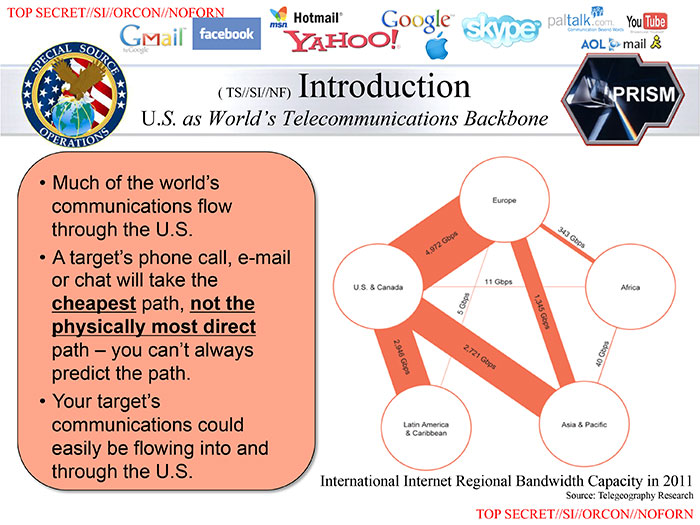
\includegraphics[scale=0.5]{Boundless.jpg}}
		\caption{ Часть презентации SOF США о PRISM и Boundless Informant, предоставленная Э.Сноуденом}
	\end{figure*} 
	\textbf{PRISM}.  Государственная программа и 	комплекс мероприятий, осуществляемых с целью  негласного массового  сбора информации, передаваемой   сетями электросвязи, принятая АНБ в 2007. Утечка данных о существовании программы стало известно в 2013 после публикации отрывков секретной презентации в   <<The Guardian>> и <<The Washington Post>>. Мощность системы оценивается в 1.7 млрд. телефонных звонков и электронных сообщений и 5 млрд. записей о местонахождении владельцев мобильных телефонов в день \cite{PRISM1} \cite{PRISM2}. %LITER https://www.theguardian.com/world/2013/jun/06/us-tech-giants-nsa-data
	%LITER https://www.washingtonpost.com/world/national-security/us-company-officials-internet-surveillance-does-not-indiscriminately-mine-data/2013/06/08/5b3bb234-d07d-11e2-9f1a-1a7cdee20287_story.html
	
	Обнародование информации о PRISM вызвало рост внимания общетсвенности на технологиях PGP, шифрованном мессенджере   Bitmessage и технологиях TOR  \cite{PRISM3}. %LITER https://www.bloomberg.com/news/articles/2013-06-27/bitmessages-nsa-proof-e-mail
	
	
	\textbf{NarusInsight}. Кластерная система шпионажа, разрабатываемая компанией Boeing для американского правительства \cite{Narus}. %LITER https://www.bloomberg.com/research/stocks/private/snapshot.asp?privcapId=59181865
	Система состоит из большого количества компьютеров, соединённых в кластер и устанавливаемых в дата-центрах провайдеров интернета в США и Западной Европе. Система предоставляет очень широкие возможности для мониторинга, перехвата, хранения и анализа больших объёмов интернет-данных: масштабирование для анализа  сверхбольших IP-сетей, real-time обработку пакетов,  глубокая обработка данных искусственным интеллектом: нормализация, корреляция, агрегация и анализ, создающие информационные модели как отдельных пользователей, так и элементов информационных систем и их протоколов и приложений с возможностью анализа моделей в реальном времени; отслеживание индивидуальных пользователей и определение используемых  ими программ коммуникации, высокая надёжность и отказоустойчивость, может использоваться для блокировки шифрованных сетей,  построена в соответствии с законами о мониторинге пользователей CALEA и ETSI.
	
	\textbf{Tempora}. Секретная программа слежения за компьютерами и коммуникационными сетями. Создана в 2011 совместными усилиями  Центра правительственной связи Великобритании и АНБ.	Широкой общественности стала известна в 2013 году, одновременно с PRISM. Перехваченные данные хранятся 3 дня, метаданные -- более 30 \cite{Tempora}. %LITER www.theatlanticwire.com/national/2013/06/uk-tempora-program/66490/
	
	
	\textbf{MUSCULAR}.    Шпионская  программа слежения, используемая Центром правительственной связи Великобритании (GCHQ) и АНБ, получившая известность благодаря Э. Сноудену в 2013, одновременно с PRISM и Tempora. GCHQ и АНБ используют программу для перехвата данных с серверов Yahoo! и Google. Для доступа к данным были тайно взломаны коммуникационные линии между Yahoo! и Google, объем перехвата составил  несколько миллионов учетных записей и информации о владельцах.  После скандала,Google заявила о начале работ над шифрованием хранимых данных \cite{MUSCULAR}. 	%LITER:https://www.washingtonpost.com/news/the-switch/wp/2013/11/04/how-we-know-the-nsa-had-access-to-internal-google-and-yahoo-cloud-data/
	%LITER https://www.washingtonpost.com/?utm_term=.54de38d6262f
	%LITER https://apps.washingtonpost.com/g/page/world/how-the-nsas-muscular-program-collects-too-much-data-from-yahoo-and-google/543/#document/p3/a129339
	%GRAPH https://upload.wikimedia.org/wikipedia/commons/f/f2/NSA_Muscular_Google_Cloud.jpg
	\begin{figure*}[h!]
		\centering{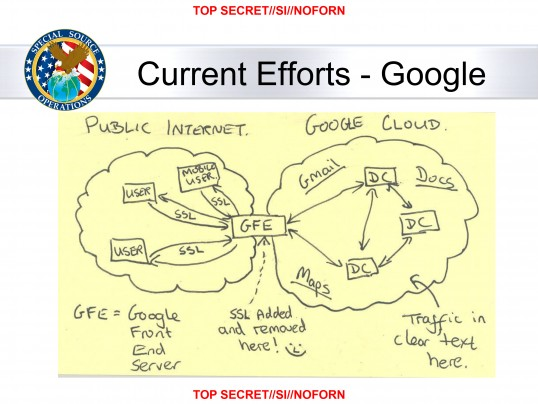
\includegraphics[scale=0.8]{Muscular.jpg}}
		\caption{ Часть презентации SOF США о MUSCULAR, предоставленная Э.Сноуденом}
	\end{figure*} 
	
	\textbf{Frenchelon}. Глобальная система радиоэлектронной разведки, тайно используемая правительством Франции. Существование системы никогда не признавалось официальными лицами Франции, однако после расследования Европейского парламента появилось множество публикаций в СМИ, доказывающих наличие такой системы. %LITER https://web.archive.org/web/20130709003259/http://www.maurizioturco.it/iniziative_politiche/echelon_dossier/banca_dati/rassegna_stampa/1998_06_06_le_point_espionn.html
	Станция слежения имелись как на территории Франции, так и в заморских владениях и бывших колониях по всему миру. Основным назначением системы являлся перехват военных и дипломатических сообщений, при этом была возможность использования системы и для слежения за гражданскими лицами. 
	
	\textbf{Onyx}. Аналогичная Frenchelon система разведки и перехвата цифровых сообщений, действующая на территории Швейцарии. Введена в эксплуатацию в 2005 году	и используется для мониторинга и хранения гражданских и военных коммуникаций: телефон, Интернет, факс с помощью системы спутников. Весь трафик пропускается через систему фильтрации контента, основанную на списке ключевых слов. В 2006 вокруг Onyx разгорелся скандал, связанный с перехваченными с помощью этой системы дипломатическими сообщениями Египта, просочившимися в прессу. Правительство Швейцарии  не подтвердило эти данные, хотя начало преследование газеты  Blick за публикацию секретных документов \cite{Onyx}. %LITER http://www.swissinfo.org/eng/search/detail/Reporters_cleared_of_revealing_military_secret.html?siteSect=881&sid=7725767&cKey=1176838959000
	%LITER http://www.blick.ch/sonntagsblick/aktuell/artikel30413
	\\
	
	
	\textbf{Российская Федерация}.  В последние несколько лет тема сбора и анализа трафика граждан, в том числе перехват и анализ переписки в интернете с целью борьбы с экстремизмом, стала невероятна остра и актуальна. Далее рассмотрены основные средства анализа и хранения трафика  в РФ, новейшие законопроекты и скандалы, связанные с защитой частной переписки. 
	
	\textbf{СОРМ}( Система технических средств для обеспечения функций оперативно-розыскных мероприятий). Согласно Закону <<О связи>> и  приказу Министерства связи № 2339 от 9 августа 2000 г., СОРМ представляет собой <<комплекс технических средств и мер, предназначенных для проведения оперативно-розыскных мероприятий в сетях телефонной, подвижной и беспроводной связи и радиосвязи>>. %LITER http://www.ispreview.ru/doc8.html
	При этом необходимо различать три поколения СОРМ:
	\begin{itemize}
		\item СОРМ-1. Система прослушивания телефонных коммуникаций, организована в 1996 году.
		\item СОРМ-2.  Система протоколирования обращений к сети Интернет. Разработана совместными усилиями ФСБ России, Госкомсвязи России, Главсвязьнадзора и ЦНИИ Связи. Организована в 2000 для прослушивания телефонных переговоров, контроля технических каналов связи.
		\item СОРМ-3. Система обеспечения сбора и долгосрочного хранения данных, получаемых от операторов  связи, АТС,  провайдеров интернет.  
	\end{itemize}

	СОРМ обязателен для всех операторов связи в РФ, иначе возможно аннулирование их лицензии \cite{SORM1}. %LITER https://rg.ru/2005/09/02/pravila-dok.html
	%GRAPH https://cdn2.img.ria.ru/images/95653/50/956535056.png
		\begin{figure*}[h!]
		\centering{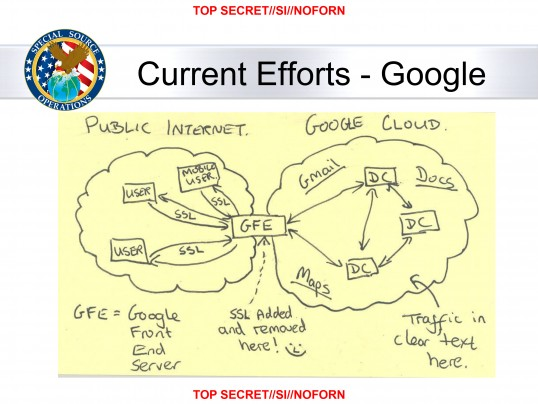
\includegraphics[scale=0.8]{Muscular.jpg}}
		\caption{ Часть презентации SOF США о MUSCULAR, предоставленная Э.Сноуденом}
	\end{figure*} 
	
	Конституция РФ (23 статья) допускает ограничение тайны связи только согласно решению суда, однако пункт 3 статьи 55 позволяет также ограничивать право на тайну связи, если << это необходимо в целях защиты основ конституционного строя, нравственности, здоровья, прав и законных интересов других лиц, обеспечения обороны страны и безопасности государства>>. Также упоминается возможность использования СОРМ до получения судебной санкции в случаях, установленных федеральными законами \cite{SORM2}. %LITER https://www.kommersant.ru/doc/863187
	
	Для непосредственного прослушивания разговоров требуется официальное судебное решение, однако для получения другой информации (  о фактах совершения вызовов) санкции суда не требуется. Более того, сотрудники ФСБ или МВД должен получить ордер, но не обязан предъявлять его оператору связи. Также, оператор не имеет права требовать ордер, если сам не имеет допуска к государственной тайне. 
	
	\textbf{Пакет Яровой}. Два законопроекта, вносящие ряд поправок в закон «О противодействии терроризму» и другие акты, касающиеся этого вопроса, и в статьи Уголовного кодекса РФ, также касающиеся антитеррора. Первая часть пакета -- это федеральный 	закон № 374-ФЗ. Данный ФЗ возлагает на операторов связи обязательство хранить и предоставлять доступ к звонкам, сообщениям и истории посещения интернет страниц своих пользователей для МВД и ФСБ. Вызвал большой общественный резонанс, так как такая база данных может попасть в третьи руки при ненадлежащем хранении и использовании. Вторая часть пакета -- федеральный закон 375-ФЗ. Данный ФЗ не настолько интересен с точки зрения данной работы, т.к не предъявляет требований, которые прямо или косвенно могут привести к нарушению тайны связи, однако все равно приведем основные идеи: ужесточение ответственности за террористическую деятельность, возможность привлекать подростков от 14 лет к уголовной ответственности за терроризм, введение понятия <<недоносительство>>.  
	
	Основная критика первого ФЗ :
	\begin{itemize}
		\item Стоимость. Создание дата-центров для хранения заявленных объемов информации может стоить до 2.2 трлн рублей для <<Большой тройки>>, при этом затраты будут возложены на абонентов, то есть реализация данного пакета приведет  к увлечению стоимости мобильной  связи и интернета \cite{Yar1}; %LITER https://www.vedomosti.ru/technology/articles/2016/08/22/653913-million-nadezhnie-ruki
		\item Эффективность. Высказываются сомнения по поводу эффективности хранения такого объема данных -- хотя это и может помочь расследованию совершенных преступлений, едва ли это сможет помочь в анализе шифрованного трафика, который будут использовать потенциальные злоумышленники для коммуникации;
		\item Потенциальные утечки. Существует  вероятность, что такие базы, хранящие личные данные, в том числе цифровую переписку, множества граждан могут быть проданы или попасть в руки злоумышленников.    
	\end{itemize}
	
	
	\textbf{Требования ФСБ к мессенджерам}. В марте 2018 ФСБ обязала организаторов распространения информации в сети предоставлять ключи шифрования в срок, не превышающий 10 дней. %LITER http://www.aif.ru/society/law/fsb_obyazala_messendzhery_predostavlyat_klyuchi_shifrovaniya_v_techenie_10_dney
	Таким образом, планируется наладить взаимодействие между силовыми ведомствами и мессенджерами  с целью анализа зашифрованных сообщений и поиска потенциальных террористов. С точки зрения данной работы, требование является трудно реализуемым: некоторые мессенджеры  не содержат ключей (Viber), другие же используют алгоритмы, которые делают приватные ключи недоступными (Telegram, протокол Диффи — Хеллмана) \cite{Yar2}. %LITER https://russian.rt.com/russia/article/499219-telegram-peredacha-fsb-klyuchi-shifrovaniya
	Также, существуют опасения, связанные с возможностью утечек переданных ключей  и попаданием последних в третьи руки, что потенциально компрометирует крупнейшие мессенджеры и их пользователей и наносит значительный экономический ущерб владельцам мессенджеров.
	
	На момент написания работы данный инцидент все еще не завершен, однако уже привел к конфронтации между РКН и руководством Telegram из-за технической невозможности передачи ключей к закрытым чатам. 
\newpage